% This file was converted to LaTeX by Writer2LaTeX ver. 1.0.2
% see http://writer2latex.sourceforge.net for more info
\documentclass[a4paper]{article}
\usepackage[utf8]{inputenc}
\usepackage[T3,T1]{fontenc}
\usepackage[slovene,english,french]{babel}
\usepackage[noenc]{tipa}
\usepackage{tipx}
\usepackage[geometry,weather,misc,clock]{ifsym}
\usepackage{pifont}
\usepackage{eurosym}
\usepackage{amsmath}
\usepackage{wasysym}
\usepackage{amssymb,amsfonts,textcomp}
\usepackage{color}
\usepackage{array}
\usepackage{supertabular}
\usepackage{hhline}
\usepackage{hyperref}
\hypersetup{pdftex, colorlinks=true, linkcolor=black, citecolor=black, filecolor=black, urlcolor=black, pdftitle=OpenWIM, pdfauthor=Ivan, pdfsubject=, pdfkeywords=}
\usepackage[pdftex]{graphicx}
\usepackage[alf,utf8,recuo=8pt]{abntex2cite}


% Text styles
\newcommand\textstyletablecaptionCar[1]{\foreignlanguage{english}{\textbf{#1}}}
% Outline numbering
\setcounter{secnumdepth}{2}
\renewcommand\thesection{\arabic{section}}
\renewcommand\thesubsection{\arabic{section}.\arabic{subsection}}
\makeatletter
\newcommand\arraybslash{\let\\\@arraycr}
\makeatother
% List styles
\newcommand\liststyleWWNumvi{%
\renewcommand\theenumi{\arabic{enumi}}
\renewcommand\theenumii{\arabic{enumii}}
\renewcommand\theenumiii{\arabic{enumiii}}
\renewcommand\labelitemi{[F0B7?]}
\renewcommand\labelenumi{\theenumi.}
\renewcommand\labelenumii{\theenumii.}
\renewcommand\labelenumiii{\theenumiii.}
}
% Page layout (geometry)
\setlength\voffset{-1in}
\setlength\hoffset{-1in}
\setlength\topmargin{2.501cm}
\setlength\oddsidemargin{2.501cm}
\setlength\textheight{24.698002cm}
\setlength\textwidth{15.999001cm}
\setlength\footskip{0.0cm}
\setlength\headheight{0cm}
\setlength\headsep{0cm}
% Footnote rule
\setlength{\skip\footins}{0.119cm}
\renewcommand\footnoterule{\vspace*{-0.018cm}\setlength\leftskip{0pt}\setlength\rightskip{0pt plus 1fil}\noindent\textcolor{black}{\rule{0.25\columnwidth}{0.018cm}}\vspace*{0.101cm}}
% Pages styles
\makeatletter
\newcommand\ps@Standard{
  \renewcommand\@oddhead{}
  \renewcommand\@evenhead{}
  \renewcommand\@oddfoot{}
  \renewcommand\@evenfoot{}
  \renewcommand\thepage{\arabic{page}}
}
\makeatother
\pagestyle{Standard}
\setlength\tabcolsep{1mm}
\renewcommand\arraystretch{1.3}
% footnotes configuration
\makeatletter
\renewcommand\thefootnote{\arabic{footnote}}
\makeatother

%\bibliographystyle{plain}
\bibliographystyle{abntex2-alf}

\def\citeay#1{\citeauthor{#1} (\citeyear{#1})} % Super!!!!!

\title{Universidade Federal de Santa Catarina}
\author{Ivan Ogassavara}
\date{2016-02-14}
\begin{document}
\clearpage\setcounter{page}{1}\pagestyle{Standard}
{\centering\selectlanguage{english}\bfseries
OpenWIM - Open Science and Weigh-in-Motion Research
\footnote{
$\copyright$ 2016, GOLTSMAN, Helio and OGASSAVARA, Ivan. Licensed under the Creative Commons Attribution 4.0 license, http://creativecommons.org/licenses/by/4.0/
}
\par}


\bigskip

\begin{flushleft}
\tablehead{}
\begin{supertabular}{m{3.8749998cm}m{3.8760002cm}m{3.8760002cm}m{3.8749998cm}}
\selectlanguage{english} Technologist researcher graduated from the Faculty Eniac, specialized in Information Systems at the Graduate Center Eniac. Experience in algorithms for moving vehicle weight estimation. &


\includegraphics[width=2.619cm,height=3.307cm]{openwim-img/openwim-img1.png}
 &

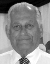
\includegraphics[width=2.619cm,height=3.307cm]{openwim-img/openwim-img2.jpg}
 &
\selectlanguage{english} Engineer researcher graduated from PUC-RJ, specialized in urban transportation planning by Massachusetts Institute of Technology - MIT. He was also one of the pioneers of the weighing area of heavy vehicles in Brazil, working since 1974 on this issue.\\
\multicolumn{2}{m{7.951cm}}{\centering
{\selectlanguage{english}\bfseries Ivan Ogassavara}\par

\centering {\selectlanguage{english} Universidade Federal de Santa Catarina}\par

\centering \selectlanguage{english} Brazil} &
\multicolumn{2}{m{7.951cm}}{\centering
{\selectlanguage{english}\bfseries Helio Goltsman}\par

\centering {\selectlanguage{english} Universidade Federal de Santa Catarina}\par

\centering \selectlanguage{english} Brazil}\\
\end{supertabular}
\end{flushleft}

\bigskip


\bigskip

{\selectlanguage{english}\bfseries
Abstract
}

{\selectlanguage{english}

Abstract ...
}


\bigskip


{\selectlanguage{english}
\textstyletablecaptionCar{Keywords:} \ Heavy
Vehicles, Weigh-in-Motion, WIM, Open Science, Open Data, Reproducibility.}


\bigskip

{\selectlanguage{english}\bfseries
\foreignlanguage{portuguese}{Resumo}}

{\selectlanguage{english}
\foreignlanguage{portuguese}{
Resumo...
}}


\bigskip

{\selectlanguage{english}
\textstyletablecaptionCar{\foreignlanguage{portuguese}{Palavras-Chaves:}}\foreignlanguage{portuguese}{
Veículos Pesados, Pesagem em Movimento, WIM, Ciência Aberta, Dados Abertos, Reprodutibilidade}}

\newpage
\section{Introduction}
{\selectlanguage{english}

Overweight heavy vehicles represent a problem related to accidents and pavement damage. The weight enforcement is very important to inhibit the overweight of these vehicles. One method that is being investigated in many parts of the world is weigh-in-motion (WIM), which has the advantage of reduced physical space required and operating with lower costs. Since the sensors can be installed on the road itself, the vehicles can be weigh without them having to slow down, hence, not delaying the road user’s journey.

Although there are many papers publicly available about weigh-in-motion, a little bit researchers publish their sources and data, which can allow a better reproduction of their experiments and results. In this context, the Open Science concept can help improve the WIM research through collaborative efforts and reproducible methods, using algorithms and data with open access.

The OpenWIM project was born upon this background as an open science initiative, to provide a WIM researchers a repository with initial structure that can then be converted into a framework for researchers to develop and test new methods and technologies.

The structure of this project was designed over some pillars:
\begin{itemize}
\item Standards;
\item Open Data;
\item Open Source;
\item Open Access;
\item Reproducibility;
\end{itemize}

The Standards pillar is based on a recompilation of standards found in the international literatures used in WIM projects. This can be a guideline to new researchers to structure their projects and can facilitate sharing data and algorithms. This standards can be about the file names, layout data structure, file format used in system integration, standard units, column name standard (in data files), algorithms style code, etc.

The Open Data pillar is based on a open repository where Weigh-in-Motion data is published. This data can be:

\begin{itemize}
\item raw data from weigh sensors;
\item raw data from inductive loop;
\item known information about the vehicle run (gross vehicle weight, speed, distance between axles, weight in each axle, vehicle category, temperature, etc.);
\item vehicle category patterns;
\item calibration data;
\item license plate images;
\item vehicle images;
\end{itemize}

The raw data from sensors and the weight information is very important to validate weigh and calibration methods. Raw data from inductive loop can help in methods like vehicle classification. The license plate images can help to test or improve methods that recognizes the license plate position and value.

The Open Source pillar is based on a repository for researchers publish his algorithms used in their research. This algorithms with a test dataset (open data) can help others in their research that allows more alternatives in their experiments. Other important key about this pillar is the informal peer-review because when other researchers can test some algorithms they can find some problem or exception or just can give some feedback.

The Open Access pillar is based on paper publishing on open repositories. This concept can allow a collaborative environment for researchers of all parts of the world to work and can increase paper citation.

The Reproducibility pillar is achieved through open access, open data and open source. To share code, explain and describe the methods, in a reproducible way, a \textit{notebook science} tool can be used. With that, the researchers can write texts, including texts with LaTeX format and algorithms; open data files; plot charts; display tables; show images; etc. Jupyter Notebooks, the most famous notebook science tool, can be used with some famous programming languages like Python, Julia, Octave, Bash, Scheme, etc.

This paper will show the idea of the OpenWIM project and its potential benefits.

\section{Open Science}\label{open-science}
Access to the academic literature (open access), data sharing (open data), and algorithms sharing (open source) are the kernel of the open science (or open research) concept \cite{article:the-open-research-value-proposition}.

The open science practices conduct the research to be more transparent \cite{dorch2015open}

The Open Access is a key to occur the Open Science \cite{margoni2016open}.

A very important governmental open science initiative is the Open Science and Research Initiative from Finland \cite{olsbo2015roadmap}

\section{OpenWIM Project}\label{open-wim}

The OpenWIM Project intend to be a central repository for data, algorithms and research. Its primaries objectives are:

\begin{itemize}
\item discussing and definition of format standards;
\item discussing and definition of open repositories;
\item offer a single point to be sharing data, code and research;
\item offer a central communication channel to discuss about WIM theme;
\item offer a social media communication to announce new and updated releases into the repository.
\end{itemize}

Standard formats is important to allow reusability of algorithms and data, consequently, that can expand the range of tests and experiments.

The repository choice is not trivial, is important know what tools are available and the number of users that know that platform. This can facilitate new researchers to contribute to the project.

Maybe more than one repository should be used, some repositories is specialized in:

\begin{itemize}
\item algorithms (i.e. GitHub\footnote{http://github.com});
\item data (i.e. Dataverse\footnote{https://dataverse.harvard.edu/});
\item images (i.e. figshare\footnote{https://figshare.com/});
\item research (i.e. Open Science Framework\footnote{https://osf.io}).
\end{itemize}

The scientific knowledge communication starting since the first phase of the scientific process, like the problem identification, until the other scientists have read the final paper \cite{leite2007scientific}.

The OpenWIM concept absorb a lot of the \textit{International Society for Weigh in Motion\footnote{http://www.is-wim.org/index.php?nm=0$\&$nsm=1$\&$lg=en}}

\subsection{Standards}\label{standards}

The Weigh-in-Motion (WIM) Systems can collect data from different kind of devices, like Automatic License Plate Recognition (ALPR), weigh sensors (piezoelectric quartz, piezoelectric ceramic, piezoelectric polymer, etc), temperature sensors, etc. So, the WIM Systems can produce a variety kind of data, like:

\begin{itemize}
\item raw sensors data;
\item estimated data, like speed, gross vehicle weight, axles weight, axles group weight, distance between axles, vehicle classification, etc;
\item environment data, like temperature, humidity, traffic condition, etc;
\item statistic data, like relative errors, etc.
\end{itemize}

In the literatures have some papers about data standards recommendations about data storage, processing, transmission and standard format \cite{tech:cost-323}, \cite{enright2011cleaning}, \cite{qu1997traffic}, \cite{elkins2008development}. These literatures can be used as the initial proposition to the data standards.

Additionally, some proceedings to clean the data are recommend before analysis stage \cite{elkins2008development}, \cite{enright2011cleaning}.


\subsection{Repositories}\label{repositories}

The main papers' index	about weigh-in-motion is at localized at the \textit{International Society for Weigh in Motion \footnote{http://www.is-wim.org/index.php?nm=3$\&$lg=en}} (IS-WIM) web site. Although, some important papers are not presented there. Some papers are stored in IS-WIM server but other papers or documents not, and so, some document could have a broken link there. 

The OpenWIM need to be supported by a platform that help the research workflows and allow storage and publishing of research products like papers, data, code, images, etc. One very interesting one is \textit{Open Science Framework\footnote{https://osf.io} (OSF)}.

One of the main idea behind the use of open science communication (publishing of all kind of research products during all phases of the research life-cycle) is maximize research reuse and reduce their costs \cite{assante2015science}.


\subsection{Dissemination}\label{dissemination}

\section{Discussion}\label{discussion}

\begin{small}
\renewcommand{\bibname}{References}
\addcontentsline{toc}{section}{\bibname}
\bibliography{openwim}
\end{small}

\end{document}
